% !TeX spellcheck = es_ES
\documentclass{article}
\usepackage[utf8]{inputenc}
\usepackage{graphicx}
\usepackage[spanish]{babel}

\title{Tarea 2 - Comparación de indices}
\author{Pablo Sanabria Q.}

\begin{document}
	\maketitle
	
	\section{Introducción}
	Existen distintas formas para indexar descriptores los cuales
	tienen el objetivo de hacer búsquedas mucho más eficientes.
	En el presente trabajo se realizó la prueba de 2 tipos de algoritmos para indexación y búsqueda de descriptores: KD-Tree y K-Means.
	\section{Metodología}
	El trabajo se dividió en tres etapas: Recopilación de información, programación y experimentación.
	\subsection{Recopilación de información}
	Para hacer un uso eficiente del tiempo de desarrollo se procedió a investigar la librería FLANN, Esta implementa los índices requeridos para nuestras pruebas, además de ciertas funciones que facilitan las pruebas a realizar.	La librería se encuentra en su página oficial\footnote{Página oficial: http://www.cs.ubc.ca/research/flann/}, junto a toda su documentación.
	
	Dentro de esta librería se dispuso a probar sus funciones y de ahí identificar las clases más importantes que permitan hacer uso de los índices requeridos.
	\subsection{Programación}
	El código fuente está dividido en varios métodos, los cuales hacen uso de la librería FLANN. Este código esta
	escrito en el lenguaje C++. Para el proceso de compilación se integró el sistema de compilación con CMake. El compilador 
	usado fue gcc, los flags activados para la compilación fueron los siguientes:
	\begin{itemize}
		\item Habilitar todas las advertencias y tratarlas como error: \texttt{-Wall -pedantic -Wextra -Werror}
		\item Obligar al compilador a usar a usar el estandar C++ 98: \texttt{-std=c++98}
		\item Habilitar las optimizaciones de código: \texttt{-O3}
	\end{itemize}	
	La parte más importante del código es la función \texttt{process\_dataset} que se encarga de procesar los archivos del dataset y query, generar las estructuras de datos necesarias para las pruebas y crear los indices. Para realizar esta tarea se ayuda de dos funciones, la primera es la función \texttt{readFile} la cual se encarga de leer el archivo y pasarlo a un \texttt{vector} y la otra función, \texttt{testPrecision}, que se encarga de hacer la prueba a un tipo de índice. Por último, la función \texttt{testPrecision} hace uso de una función \texttt{compareWithGroundTruth} que se encarga de comparar el resultado de la búsqueda de vecino más cercano con el ground truth, calcular la precisión y dar a saber el tiempo de ejecución de la búsqueda.
	
	El método \texttt{main} lo único que hace es leer los argumentos que son necesarios para la ejecución de las pruebas y llamar a la versión correcta de la función \texttt{process\_dataset}.
	
	\subsection{Experimentación}
	Para la experimentación se procedió a probar el programa en un computador que tiene un procesador de 3.4GHz y memoria de 16Gb, este opera bajo el sistema operativo Linux. Las pruebas se realizaron con cuatro tipos de descriptores:
	\begin{itemize}
		\item \textbf{Imagen reducida}: 144 dimensiones, enteros de un byte
		\item \textbf{Ordinal Measurement}: 144 dimensiones, enteros de un byte
		\item \textbf{Edge histogram}: 160 dimensiones, decimales de 4 bytes
		\item \textbf{Audio}: 160 dimensiones, decimales de 4 bytes
	\end{itemize}
	Para cada descriptor se pasó al programa el dataset y el query, junto al tipo de dato esperado y la cantidad de dimensiones. La salida del programa fue redirigida a un archivo de texto para un posterior análisis.
	
	Cada archivo de texto fue posteriormente postprocesado en un programa de Hojas de Cálculo (Open Office) para el posterior análisis. Como una aclaración adicional. A cada gráfica se agrega una línea (excepto para el descriptor Edge Histogram) el cual es el tiempo de ejecución para la búsqueda lineal.
	
	\section{Resultados}
	Posterior a la ejecución del programa y el postprocesado de las salidas de este se obtuvo los siguientes resultados:
	\begin{figure}
		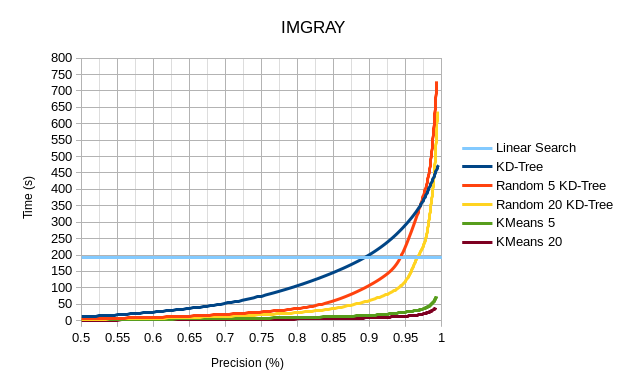
\includegraphics[width=\linewidth]{imgray.png}
		\caption{Resultados imagen reducida}
	\end{figure}
	\begin{figure}
		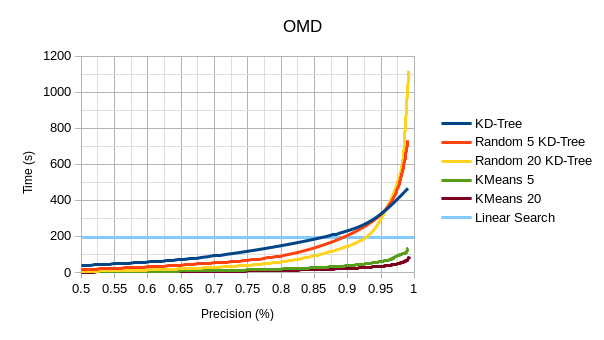
\includegraphics[width=\linewidth]{omd.png}
		\caption{Resultados Ordinal Measurement}
	\end{figure}
	\begin{figure}
		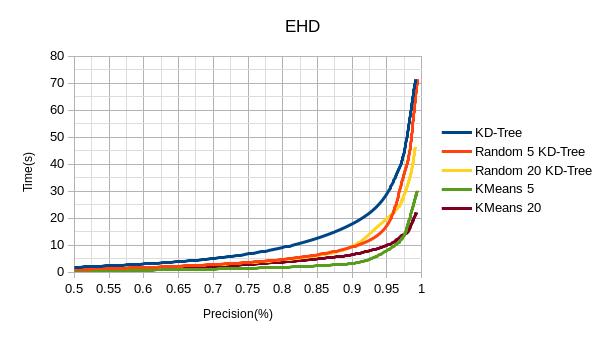
\includegraphics[width=\linewidth]{ehd.png}
		\caption{Resultados Edge histogram}
	\end{figure}
	\begin{figure}
		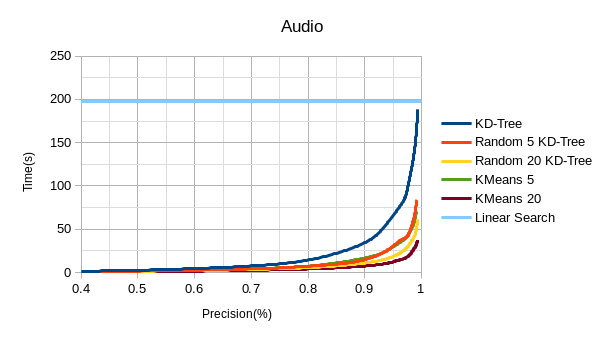
\includegraphics[width=\linewidth]{audio.png}
		\caption{Resultados Audio}
	\end{figure}
	Los resultados en general son de cierta manera esperables. Se puede observar que el KD-Tree, en cualquiera de sus formas empieza a empeorar de forma súbita cuando es necesaria una mayor precisión del resultado. Mientras que los K-Means se comportaron de muy buena forma en terminos de tiempo de ejecución para cuando se requería mayor precisión.
	
	De forma individial, para el descriptor de imagen reducida puede observarse que de lejos los K-Means funcionan de manera excepcional al pedirles mayor precisión y mientras tanto los KD-Trees tienden a tener una explosión en tiempo de ejecución cada vez que se les pide tener mayor precisión. Es interesante hacer notar que solamente un KD-Tree tiene mejor rendimiento que tener varios KD-Trees, esto debe ser causado por que no tiene que recorrer varios árboles los cuales podrían contribuir en el tiempo de ejecución debido a la lógica del algoritmo. Cabe también resaltar que este comportamiento igualmente se puede notar en el descriptor Ordinal Measurement.
	
	En el caso del descriptor Edge Histogram puede hacerse notar que ninguno de los índices tienen una explosión abrupta en el tiempo de ejecución al pedirles más precisión, además de que ningun índice llega a superar en tiempo de ejecución a la búsqueda lineal (ni siquiera se acerca a este tiempo). Nuevamente en este descriptor los K-Means tienen mejor rendimiento que los KD-Trees
	
	Para el descriptor de audio se puede notar que los KD-Trees aleatorios y los K-Means tienen un comportamiento similar, mientras que un KD-Tree empieza a tener una explosión en tiempo de ejecución pero sin sobrepasar el límite del tiempo de la búsqueda lineal (aunque esta bastante cerca)
	
	Es interesante observar que los Kd-Tree a pesar de ser teoricamente rápidos en la búsqueda del vecino más cercano en este tipo de dataset presente problemas en tiempo de ejecución, esto puede ser debido a la alta dimensionalidad de los descriptores.
	
	\section{Conclusiones}
	Por los resultados obtenidos, se podría decir que en la mayoria de los casos el indice de tipo K-Means tiene un mejor rendimiento para buscar el vecino más cercano dentro de un conjunto de descriptores de alta dimensionalidad. La causa probable del mal rendimiento de los KD-Trees es la dimensionalidad ya que al tener tantas dimensiones, provoca que los KD-Trees tengan demasiadas intersecciones y haciendo que la búsqueda del vecino más cercano se vuelva lineal, o incluso peor que esta.
	
	Por lo que se vio en los resultados, igualmente podría afirmarse que para este tipo de problemas el descriptor Edge Historial puede presentar un mejor rendimiento y que a cierto nivel, es independiente al tipo de indice que se pueda elegir.
\end{document}